\newpage
\section{Application à un drive oscillant}
\subsection{Préliminaires}
Un drive est un laser qu'on envoie sur un transmon afin de manipuler son état. Contrairement à un pulse qui ne dure qu'un bref instant, un drive est appliqué plus longtemps de manière à avoir une rentrée d'énergie prolongée. Ici, le drive oscille et son application occasionne au transmon des changements de niveaux d'énergie. Le qubit évolue donc avec un hamiltonien dépendant du temps. Dans un tel contexte, ce dernier correspond à  

\begin{equation}
    H(t) = H_0 + V(t)
\end{equation}

où, dans sa base d'états propres, $H_0 = \sum_{k} \lambda_k \ket{k}\bra{k}$ correspond aux énergies du transmon quand on le laisse tranquille et $V(t) = X\cos(\omega t)$, pour un opérateur quelconque $X$, correspond à la modification due au drive. En décomposant le cosinus en exponentielles complexes, 

\begin{equation*}
    H(t) = H_0 + X\left(\frac{e^{i \omega t} + e^{-i\omega t}}{2}\right)
\end{equation*}

On s'attarde à l'opérateur d'évolution dans cette situation. Pour une variation infime de temps et en utilisant (2.1), on trouve (et ça fait peur)

\begin{equation*}
    U(t+\delta t, t) = \sum_{n=0}^{\infty} (-i)^n \int_{t}^{t+\delta t}\int_{t}^{t_n}...\int_{t}^{t_2}H(t_n)...H(t_1)dt_1 ... dt_n
\end{equation*}
\begin{equation*}
    = \sum_{n=0}^{\infty} (-i)^n \int_{t}^{t+\delta t}\int_{t}^{t_n}...\int_{t}^{t_2}\left(H_0 + 
    V(t_n)\right)...\left(H_0 + V(t_1)\right)dt_1 ... dt_n
\end{equation*}
\begin{equation*}
    = \sum_{n=0}^{\infty} (-i)^n \int_{t}^{t+\delta t}\int_{t}^{t_n}...\int_{t}^{t_2} \left(H_0...H_0 + H_0...H_0V(t_1) + ... + V(t_n)H_0...H_0 + ... + V(t_n)...V(t_1)\right)dt_1 ... dt_n
\end{equation*}
\begin{equation}
    = \sum_{n=0}^{\infty} \int_{t}^{t+\delta t}\int_{t}^{t_n}...\int_{t}^{t_2} (-i)^n H_0...H_0 dt_1...dt_n + ... + \sum_{n=0}^{\infty} \int_{t}^{t+\delta t}\int_{t}^{t_n}...\int_{t}^{t_2}(-i)^n V(t_n)...V(t_1) dt_1...dt_n
\end{equation}

On peut voir que la distribution des termes correspond à l'ensemble des combinaisons de $n$ opérateurs où on choisit soit $H_0$ ou $V(t)$ pour chacun d'eux. Il y a donc au total $2^n$ termes, chacun de $n$ opérateurs et pouvant alterner entre des suites de $H_0$ ou de $V(t)$ de différentes longueurs. Graphiquement, on peut représenter la génération des combinaisons par la figure 2 où chacune d'entre elles correspond à une branche différente de l'arbre.

\begin{figure}[H]
    \centering
     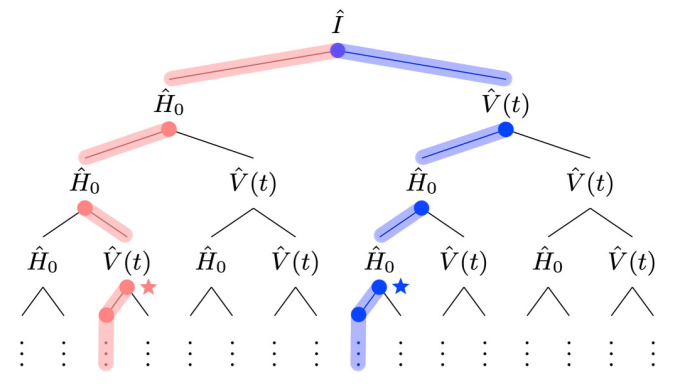
\includegraphics[width=0.45\textwidth]{images/ch2/embranchements.png}
    \caption{Arbre permettant de générer l'ensemble des combinaisons}
\end{figure}

\subsection{Dérivation (partie 1)}
On considère maintenant $n$ comme étant le nombre de $V(t)$ présents dans chaque terme de (2.2) et on omet temporairement les indices $V(t_j)$ pour éviter de se mélanger avec l'ancienne écriture. Il ne s'agit plus du même $n$ que dans (2.2) et il faut alors un nouveau moyen d'écrire tout cela avec ce changement de variables. Pour se faire, on introduit les $m_i$ qui indiquent combien d'applications de $H_0$ il y a avant une application d'un $V(t)$. Par exemple,

\begin{equation*}
    H_0V(t)H_0H_0 = (H_0)^1V(t)(H_0)^2 = (H_0)^{m_1}V(t)(H_0)^{m_0} \implies m_0 = 2, m_1 = 1
\end{equation*}
\begin{equation*}
    V(t)V(t) = (H_0)^0V(t)(H_0)^0V(t)(H_0)^0 \implies m_0 = m_1 = m_2 = 0
\end{equation*}

En général, ils sont indexés de $m_0$ à $m_n$, car pour un nombre $n$ de $V(t)$, on peut avoir jusqu'à $n+1$ blocs $H_0...H_0$ ayant des longueurs différentes.

\begin{equation*}
    \underline{H_0H_0}V(t) : \text{ 1 bloc, } \underline{H_0}V(t)\underline{H_0} : \text{ 2 blocs, } V(t)\underline{H_0H_0} : \text{ 1 bloc}
\end{equation*}



Cependant, chaque terme de (2.2) a une somme infinie. Ainsi, ces blocs peuvent être arbitrairement longs, faisant en sorte que les $m_i$ peuvent prendre des valeurs entre 0 et l'infini. Il est plus concis de les mettre dans un vecteur $\boldsymbol{m} = \left[m_n, ..., m_0\right] \in \mathbb{Z}^{n+1}_+$. Ainsi, on peut écrire toute chaîne d'opérateurs comme 

\begin{equation}
    (H_0)^{m_n}V(t)(H_0)^{m_{n-1}}V(t)...(H_0)^{m_1}V(t)(H_0)^{m_0}
\end{equation}

dont on obtient sa longueur $M$ (le nombre total d'opérateurs) grâce à 

\begin{equation}
    M = \left(\sum_{i=0}^{n}m_i\right) + n
\end{equation}

\subsection{Dérivation (partie 2)}
La prochaine étape est maintenant de retrouver les indices dans les $V(t)$ avec notre nouvelle notation. On sait déjà qu'il y aura $n$ opérateurs $V(t)$, mais on doit pouvoir retrouver leur positionnement dans la chaîne d'opérateurs. On peut simplement compter combien il y a de $H_0$ et d'autres $V(t)$ avant celui qui nous intéresse. Par exemple, pour $n=2$, on pourrait avoir la chaîne

\begin{equation*}
    H_0V(t)H_0V(t)H_0 \implies \boldsymbol{m} = \left[1, 1, 1\right]
\end{equation*}

Le premier $V(t)$ s'applique nécessairement après $m_0 = 1$ opérateur $H_0$. Le deuxième s'applique nécessairement après $m_0 = 1$ opérateur $H_0$, un $V(t)$ puis $m_1 = 1$ opérateur $H_0$. Si $p \in \left[1..n\right]$ est une variable qui passe au travers des $n$ opérateurs $V(t)$, alors il est facile d'avoir l'indexage $V(t_{l(p)})$ où

\begin{equation}
    l(p) = \left(\sum_{j=0}^{p-1}m_j\right) + p
\end{equation}

Pour reprendre l'exemple, 

\begin{equation*}
    H_0V(t_{l(2)})H_0V(t_{l(1)})H_0 = H_0V(t_{m_1 + m_0 + 2})H_0V(t_{m_0 + 1})H_0 = H_0V(t_4)H_0V(t_2)H_0
\end{equation*}

comme on aurait dans (2.2).

\subsection{Dérivation (partie 3)}
Ensuite, on étend les $V(t_{l(p)})$ selon leur définition qu'on rappelle ici.

\begin{equation*}
    V(t_{l(p)}) = X\left(\frac{e^{i\omega t_{l(p)}} + e^{-i\omega t_{l(p)}}}{2}\right)
\end{equation*}

Toujours avec le même exemple,

\begin{equation*}
    H_0V(t_4)H_0V(t_2)H_0 = \left(\frac{e^{i\omega t_4} + e^{-i\omega t_4}}{2}\right)\left(\frac{e^{i\omega t_2} + e^{-i\omega t_2}}{2}\right)H_0XH_0XH_0 
\end{equation*}
\begin{equation*}
    = \frac{1}{2^2}\left(e^{i\omega t_2}e^{i\omega t_4} + e^{i\omega t_2}e^{-i\omega t_4} + e^{-i\omega t_2}e^{i\omega t_4} + e^{-i\omega t_2}e^{-i\omega t_4}\right)H_0XH_0XH_0
\end{equation*}

On introduit maintenant le vecteur à $n$ dimensions $\boldsymbol{\omega}_n$ dont chacun de ses éléments peut soit être $+\omega$ ou $-\omega$. On peut aller chercher l'élément $i$ par $\boldsymbol{\omega}_n[i]$. Pour un $n$ donné, on voit qu'il en existe $2^n$ différents qu'on rassemble dans $\left\{\boldsymbol{\omega}_n\right\}$. Par exemple, 

\begin{equation*}
    \left\{\boldsymbol{\omega}_2\right\} = \left\{\left[+\omega, +\omega\right], \left[+\omega, -\omega\right], \left[-\omega, +\omega\right], \left[-\omega, -\omega\right]\right\}    
\end{equation*}

On peut alors réécrire

\begin{equation*}
    H_0V(t_4)H_0V(t_2)H_0 = \frac{1}{2^2}\sum_{\left\{\boldsymbol{\omega}_2\right\}}\left(\prod_{p=1}^{2}e^{i\boldsymbol{\omega}_2[p]t_{l(p)}} H_0XH_0XH_0\right)
\end{equation*}

Ainsi, pour une chaîne arbitraire, (2.3) peut être réécrit de la manière suivante.

\begin{equation}
    \frac{1}{2^n}\sum_{\left\{\boldsymbol{\omega}_n\right\}}\left(\prod_{p=1}^{n}e^{i\boldsymbol{\omega}_n[p]t_{l(p)}} (H_0)^{m_n}X ... X(H_0)^{m_0}\right)
\end{equation}

\subsection{Dérivation (partie 4)}
Il est maintenant temps de remettre les précédentes parties dans le contexte de (2.2). On reconstruit partie par partie. D'abord, en ne considérant que les intégrales d'un seul terme, on se retrouve grâce à notre précédente trouvaille avec

\begin{equation*}
    \int_{t}^{t + \delta t}\int_{t}^{t_M}...\int_{t}^{t_2} (-i)^M \left(\frac{1}{2^n}\sum_{\left\{\boldsymbol{\omega}_n\right\}}\left(\prod_{p=1}^{n} e^{i\boldsymbol{\omega}_n[p]t_{l(p)}} (H_0)^{m_n}X...X(H_0)^{m_0}\right)\right)dt_1 ... dt_M
\end{equation*}
\begin{equation*}
    = \frac{1}{2^n}\sum_{\left\{\boldsymbol{\omega}_n\right\}}\left(\int_{t}^{t + \delta t}\int_{t}^{t_M}...\int_{t}^{t_2} (-iH_0)^{m_n}X...X(-iH_0)^{m_0} \cdot (-i)^n \prod_{p=1}^{n}e^{i\boldsymbol{\omega}_n[p]t_{l(p)}} dt_1 ... dt_M\right)
\end{equation*}

Il y a ensuite une somme infinie pour chaque terme qu'on absorbe dans les différentes longueurs $m_i$. On doit donc ajouter

\begin{equation*}
    \frac{1}{2^n}\sum_{\left\{\boldsymbol{\omega}_n\right\}}\sum_{\boldsymbol{m} \in \mathbb{Z}^{n+1}_+}\left(\int_{t}^{t + \delta t}\int_{t}^{t_M}...\int_{t}^{t_2} (-iH_0)^{m_n}X...X(-iH_0)^{m_0} \cdot (-i)^n \prod_{p=1}^{n}e^{i\boldsymbol{\omega}_n[p]t_{l(p)}} dt_1 ... dt_M\right)
\end{equation*}

Puis, on doit sommer la précédente équation pour tous les nombres $n$ de $V(t)$.

\begin{equation*}
    U(t+\delta t, t) = \sum_{n=0}^{\infty}\sum_{\left\{\boldsymbol{\omega}_n\right\}}\frac{1}{2^n}\sum_{\boldsymbol{m} \in \mathbb{Z}^{n+1}_+}\left(\int_{t}^{t + \delta t}\int_{t}^{t_M}...\int_{t}^{t_2} (-iH_0)^{m_n}X...X(-iH_0)^{m_0} \cdot (-i)^n \prod_{p=1}^{n}e^{i\boldsymbol{\omega}_n[p]t_{l(p)}} dt_1 ... dt_M\right)
\end{equation*}

\subsection{Dérivation (dernière partie)}
Finalement, on procède simplement à un changement de variables $t_i^{'} = t_i - t$. Ainsi, 

\begin{equation*}
    dt_i^{'} = dt_i - dt = dt_i    
\end{equation*}
\begin{equation*}
    t_i = t_i^{'} + t
\end{equation*}
\begin{equation*}
    t_i \in \left[t, t_j\right] \implies t_i^{'} \in [0, t_j^{'}]
\end{equation*}

nous donnent tout ce qu'il faut pour faire le changement de variables.

\begin{equation*}
    U(t+\delta t, t) = \sum_{n=0}^{\infty}\sum_{\left\{\boldsymbol{\omega}_n\right\}}\frac{1}{2^n}\sum_{\boldsymbol{m} \in \mathbb{Z}^{n+1}_+}\left(\int_{0}^{\delta t}\int_{0}^{t_M^{'}}...\int_{0}^{t_2^{'}} (-iH_0)^{m_n}X...X(-iH_0)^{m_0} \cdot (-i)^n \prod_{p=1}^{n}e^{i\boldsymbol{\omega}_n[p](t_{l(p)}^{'} + t)} dt_1^{'} ... dt_M^{'}\right)
\end{equation*}
\begin{equation*}
    = \sum_{n=0}^{\infty}\sum_{\left\{\boldsymbol{\omega}_n\right\}}\left(\prod_{p=1}^{n}e^{i\boldsymbol{\omega}_n[p]t}\right)\frac{1}{2^n}\sum_{\boldsymbol{m} \in \mathbb{Z}^{n+1}_+}\left(\int_{0}^{\delta t}\int_{0}^{t_M^{'}}...\int_{0}^{t_2^{'}} (-iH_0)^{m_n}X...X(-iH_0)^{m_0} \cdot (-i)^n \prod_{p=1}^{n}e^{i\boldsymbol{\omega}_n[p]t_{l(p)}^{'}} dt_1^{'} ... dt_M^{'}\right)
\end{equation*}
\begin{equation*}
    = \sum_{n=0}^{\infty}\sum_{\left\{\boldsymbol{\omega}_n\right\}}e^{i\sum_{p=1}^{n}\boldsymbol{\omega}_n[p]t}\frac{1}{2^n}\sum_{\boldsymbol{m} \in \mathbb{Z}^{n+1}_+}\left(\int_{0}^{\delta t}\int_{0}^{t_M^{'}}...\int_{0}^{t_2^{'}} (-iH_0)^{m_n}X...X(-iH_0)^{m_0} \cdot (-i)^n \prod_{p=1}^{n}e^{i\boldsymbol{\omega}_n[p]t_{l(p)}^{'}} dt_1^{'} ... dt_M^{'}\right)
\end{equation*}

Ce n'est pas très beau, alors on définit

\begin{equation}
    S^{(n)}_{\boldsymbol{m}}(\boldsymbol{\omega}_n, \delta t) = \int_{0}^{\delta t}\int_{0}^{t_M^{'}}...\int_{0}^{t_2^{'}} (-iH_0)^{m_n}X...X(-iH_0)^{m_0} \cdot (-i)^n \prod_{p=1}^{n}e^{i\boldsymbol{\omega}_n[p]t_{l(p)}^{'}} dt_1^{'} ... dt_M^{'}
\end{equation}
\begin{equation}
    S^{(n)}(\boldsymbol{\omega}_n, \delta t) = \frac{1}{2^n}\sum_{\boldsymbol{m} \in \mathbb{Z}^{n+1}_+} S^{(n)}_{\boldsymbol{m}}(\boldsymbol{\omega}_n, \delta t)
\end{equation}
\begin{equation}
    U^{(n)}(t + \delta t, t) = \sum_{\left\{\boldsymbol{\omega}_n\right\}}e^{i\sum_{p=1}^{n}\boldsymbol{\omega}_n[p]t}S^{(n)}(\boldsymbol{\omega}_n, \delta t)
\end{equation}

de sorte que 

\begin{equation}
    U(t+\delta t, t) = \sum_{n=0}^{\infty}U^{(n)}(t+\delta t, t)
\end{equation}

% \subsection{Réécriture}
% Par (1.12),
% \begin{equation*}
%     S^{(n)}_{\boldsymbol{m}}(\boldsymbol{\omega}_n, \delta t) = \int_{0}^{\delta t}\int_{0}^{t_M^{'}}...\int_{0}^{t_2^{'}} (-iH_0)^{m_n}X...X(-iH_0)^{m_0} \cdot (-i)^n \prod_{p=1}^{n}e^{i\boldsymbol{\omega}_n[p]t_{l(p)}^{'}} dt_1^{'} ... dt_M^{'}
% \end{equation*}
% \begin{equation*}
%     = \frac{1}{M!}\int_{0}^{\delta t}...\int_{0}^{\delta t} \mathcal{T}\left[(-iH_0)^{m_n}X...X(-iH_0)^{m_0} \cdot (-i)^n \prod_{p=1}^{n}e^{i\boldsymbol{\omega}_n[p]t_{l(p)}^{'}}\right] dt_1^{'} ... dt_M^{'}
% \end{equation*}

% Comme les matrices sont indépendantes du temps et que les exponentielles dépendantes du temps sont des fonctions commutatives, $\mathcal{T}$ ne fait rien.

% \begin{equation*}
%     S^{(n)}_{\boldsymbol{m}}(\boldsymbol{\omega}_n, \delta t) = \frac{1}{M!}\int_{0}^{\delta t}...\int_{0}^{\delta t}(-iH_0)^{m_n}X...X(-iH_0)^{m_0} \cdot (-i)^n \prod_{p=1}^{n}e^{i\boldsymbol{\omega}_n[p]t_{l(p)}^{'}} dt_1^{'} ... dt_M^{'}
% \end{equation*}
% \begin{equation*}
%     = \frac{1}{M!}\int_{0}^{\delta t}...\int_{0}^{\delta t}\left(-i\sum_{k^{(n)}}\lambda_{k^{(n)}}\ket{k^{(n)}}\bra{k^{(n)}}\right)^{m_n}X...X\left(-i\sum_{k^{(0)}}\lambda_{k^{(0)}}\ket{k^{(0)}}\bra{k^{(0)}}\right)^{m_0} \cdot (-i)^n \prod_{p=1}^{n}e^{i\boldsymbol{\omega}_n[p]t_{l(p)}^{'}} dt_1^{'} ... dt_M^{'}
% \end{equation*}
% \begin{equation*}
%     = \frac{1}{M!}\sum_{k^{(n)}, ..., k^{(0)}}\int_{0}^{\delta t}...\int_{0}^{\delta t}\left(-i\lambda_{k^{(n)}}\right)^{m_n}...\left(-i\lambda_{k^{(0)}}\right)^{m_0} \bra{k^{(n)}}X\ket{k^{(n-1)}}...\bra{k^{(1)}}X\ket{k^{(0)}} \ket{k^{(n)}}\bra{k^{(0)}}
% \end{equation*}
% \begin{equation*}
%     \cdot (-i)^n \prod_{p=1}^{n}e^{i\boldsymbol{\omega}_n[p]t_{l(p)}^{'}} dt_1^{'} ... dt_M^{'}
% \end{equation*}






\subsection{Calcul de l'ordre 0}
On calcule explicitement l'ordre 0, soit $U^{(0)}(t+\delta t, t)$ la branche la plus à gauche dans la figure 2 où la chaîne d'opérateurs ne contient que des $H_0$. Ici, $\boldsymbol{m} = [m_0]$ et $\left\{\boldsymbol{\omega}_0\right\}$ est vide. Dès lors,

\begin{equation*}
    S^{(0)}_{\boldsymbol{m}}(\boldsymbol{\omega}_0, \delta t) = \int_{0}^{\delta t}\int_{0}^{t_{m_0}^{'}}...\int_{0}^{t_2^{'}} (-iH_0)^{m_0}dt_1^{'}...dt_{m_0}^{'} = \frac{(-iH_0)^{m_0}}{m_0!}\int_{0}^{\delta t}...\int_{0}^{\delta t}dt_1^{'}...dt_{m_0}^{'} = \frac{(-iH_0\int_{0}^{\delta t}dt^{'})^{m_0}}{m_0!}
\end{equation*}
\begin{equation*}
    = \frac{(-iH_0\delta t)^{m_0}}{m_0!}
\end{equation*}

où on a utilisé le même truc qu'avec les $J_n$ pour changer les bornes d'intégration. Par la suite,

\begin{equation*}
    S^{(0)}(\boldsymbol{\omega}_0, \delta t) = \frac{1}{2^0}\sum_{\boldsymbol{m} \in \mathbb{Z}^{0+1}_{+}}S^{(0)}_{\boldsymbol{m}}(\boldsymbol{\omega}_0, \delta t) = \sum_{m_0=0}^{\infty}\frac{(-iH_0\delta t)^{m_0}}{m_0!} = e^{-iH_0\delta t}
\end{equation*}

Comme $\left\{\boldsymbol{\omega}_0\right\}$ est vide, on obtient finalement

\begin{equation*}
    U^{(0)}(t+\delta t, t) = e^{-iH_0\delta t}
\end{equation*}

Le résultat a du sens, car on a seulement des opérateurs indépendants du temps. Donc, on s'attend à ce que l'opérateur d'évolution soit de la même forme que (1.3), ce qui est le cas. De manière équivalente, on peut aussi faire le précédent calcul avec la définition $H_0 = \sum_{k}\lambda_k \ket{k}\bra{k}$. Ce qui suit est évident, car $H_0$ est diagonal dans sa base d'états propres.

\begin{equation*}
    S^{(0)}(\boldsymbol{\omega}_0, \delta t) = \sum_{m_0 = 0}^{\infty}\frac{(-iH_0\delta t)^{m_0}}{m_0!} = \sum_{m_0 = 0}^{\infty}\frac{(-i\sum_{k}\lambda_k \ket{k}\bra{k}\delta t)^{m_0}}{m_0!} = \sum_{k}\sum_{m_0 = 0}^{\infty}\frac{(-i\lambda_k\delta t)^{m_0}}{m_0!}\ket{k}\bra{k} = \sum_{k}e^{-i\lambda_k\delta t}\ket{k}\bra{k}
\end{equation*}

\subsection{Calcul de l'ordre 1}
On s'attarde ici aux branches avec un seul $V(t)$ à quelque part dans la séquence d'opérateurs, ce qu'on calcule par $ U^{(1)}(t+\delta t, t)$. On sait que $\boldsymbol{m} = [m_1, m_0]$ et que $\left\{\boldsymbol{\omega}_1\right\} = \left\{[+\omega], [-\omega]\right\}$. Ainsi, 

\begin{equation*}
    S^{(1)}_{\boldsymbol{m}}(\boldsymbol{\omega}_1, \delta t) = -i\int_{0}^{\delta t}\int_{0}^{t_M^{'}}... \int_{0}^{t_2^{'}}(-iH_0)^{m_1}X(-iH_0)^{m_0} e^{i\boldsymbol{\omega}_1[1]t^{'}_{l(1)}}dt_1^{'} ... dt_M^{'}
\end{equation*}
\begin{equation*}
    = -i\int_{0}^{\delta t}\int_{0}^{t_M^{'}}... \int_{0}^{t_2^{'}}(-iH_0)^{m_1}X(-iH_0)^{m_0} e^{i\boldsymbol{\omega}_1[1]t^{'}_{m_0+1}}dt_1^{'} ... dt_M^{'}
\end{equation*}
\begin{equation*}
    = -i\int_{0}^{\delta t}dt^{'}_M\int_{0}^{t_M^{'}}dt^{'}_{M-1}...\int_{0}^{t^{'}_{m_0 + 3}}dt^{'}_{m_0 + 2}\int_{0}^{t^{'}_{m_0 + 2}}(-iH_0)^{m_1}Xe^{i\boldsymbol{\omega}_1[1]t^{'}_{m_0+1}}(-iH_0)^{m_0}  dt^{'}_{m_0 + 1} \int_{0}^{t^{'}_{m_0 + 1}}dt^{'}_{m_0}... \int_{0}^{t_2^{'}}dt_1^{'}
\end{equation*}







% Sachant dans ce cas que $M = m_0 + m_1 + 1 \implies m_0 + 1 = M-m_1$,

% \begin{equation*}
%     S^{(1)}_{\boldsymbol{m}}(\boldsymbol{\omega}_1, \delta t) = -i (-iH_0)^{m_1}X
%     \int_{0}^{\delta t}\int_{0}^{t_M^{'}}... \int_{0}^{t_2^{'}}(-iH_0)^{m_0} e^{i\boldsymbol{\omega}_1[1]t^{'}_{M-m_1}}dt_1^{'} ... dt_M^{'}
% \end{equation*}
% \begin{equation*}
%     = -i (-iH_0)^{m_1}X
%     \int_{0}^{\delta t}dt_M^{'} ... \int_{0}^{t^{'}_{M-m_1+1}}e^{i\boldsymbol{\omega}_1[1]t^{'}_{M-m_1}} dt_{M-m_1}^{'}\int_{0}^{t^{'}_{M-m_1}}... \int_{0}^{t_2^{'}}(-iH_0)^{m_0} dt_1^{'} ... dt_{M - m_1 - 1}^{'}
% \end{equation*}

De là,

\begin{equation*}
    S^{(1)}(\boldsymbol{\omega}_1, \delta t) = 
\end{equation*}
\begin{equation*}
    = \frac{-i}{2}\sum_{m_1,m_0 = 0}^{\infty} \int_{0}^{\delta t}dt^{'}_M...\int_{0}^{t^{'}_{m_0 + 3}}dt^{'}_{m_0 + 2}\int_{0}^{t^{'}_{m_0 + 2}}(-iH_0)^{m_1}Xe^{i\boldsymbol{\omega}_1[1]t^{'}_{m_0+1}}(-iH_0)^{m_0}  dt^{'}_{m_0 + 1} \int_{0}^{t^{'}_{m_0 + 1}}dt^{'}_{m_0}... \int_{0}^{t_2^{'}}dt_1^{'}
\end{equation*}
\begin{equation*}
    = \frac{-i}{2}\sum_{m_1= 0}^{\infty}\int_{0}^{\delta t}dt^{'}_M...\int_{0}^{t^{'}_{m_0 + 3}}dt^{'}_{m_0 + 2}\int_{0}^{t^{'}_{m_0 + 2}}(-iH_0)^{m_1}Xe^{i\boldsymbol{\omega}_1[1]t^{'}_{m_0+1}}dt^{'}_{m_0 + 1} \sum_{m_0 = 0}^{\infty} \frac{(-iH_0)^{m_0}}{m_0!} \left(\int_{0}^{t^{'}_{m_0+1}}dt\right)^{m_0}
\end{equation*}
\begin{equation*}
    = \frac{-i}{2}\sum_{m_1= 0}^{\infty}\int_{0}^{\delta t}dt^{'}_M...\int_{0}^{t^{'}_{m_0 + 3}}dt^{'}_{m_0 + 2}\int_{0}^{t^{'}_{m_0 + 2}}(-iH_0)^{m_1}Xe^{i\boldsymbol{\omega}_1[1]t^{'}_{m_0+1}} e^{-iH_0 t^{'}_{m_0 +1}}dt^{'}_{m_0 + 1}
\end{equation*}



% \begin{equation*}
%     \frac{1}{2} \sum_{m_1 = 0}^{\infty}\sum_{m_0 = 0}^{\infty}\left(-i (-iH_0)^{m_1}X
%     \int_{0}^{\delta t}dt_M^{'} ... \int_{0}^{t^{'}_{M-m_1+1}}e^{i\boldsymbol{\omega}_1[1]t^{'}_{M-m_1}} dt_{M-m_1}^{'}\int_{0}^{t^{'}_{M-m_1}}... \int_{0}^{t_2^{'}}(-iH_0)^{m_0} dt_1^{'} ... dt_{M - m_1 - 1}^{'}\right)
% \end{equation*}
% \begin{equation*}
%     = \frac{-i}{2}\sum_{m_1 = 0}^{\infty}(-iH_0)^{m_1}X\int_{0}^{\delta t}dt^{'}_M ... \int_{0}^{t^{'}_{M-m_1+1}}e^{i\boldsymbol{\omega}_1[1]t^{'}_{M-m_1}} dt_{M-m_1}^{'}\sum_{m_0 = 0}^{\infty}\int_{0}^{t^{'}_{M-m_1}}... \int_{0}^{t_2^{'}}(-iH_0)^{m_0} dt_1^{'} ... dt_{M - m_1 - 1}^{'}
% \end{equation*}

% On a déjà rencontré à l'ordre 0 ce qui se trouve à droite de la somme infinie sur $m_0$. Il y a en effet $m_0$ intégrales à la droite de cette somme. Alors, on écrit

% \begin{equation*}
%     S^{(1)}(\boldsymbol{\omega}_1, \delta t) = \frac{-i}{2}\sum_{m_1 = 0}^{\infty}(-iH_0)^{m_1}X\int_{0}^{\delta t}dt^{'}_M ... \int_{0}^{t^{'}_{M-m_1+1}}e^{i\boldsymbol{\omega}_1[1]t^{'}_{M-m_1}} dt_{M-m_1}^{'}S^{(0)}(\boldsymbol{\omega}_0, t^{'}_{M-m_1})
% \end{equation*}
% \begin{equation*}
%     = \frac{-i}{2}\sum_{m_1 = 0}^{\infty}(-iH_0)^{m_1}X\int_{0}^{\delta t}dt^{'}_M ... \int_{0}^{t^{'}_{M-m_1+1}}e^{i\boldsymbol{\omega}_1[1]t^{'}_{M-m_1}} dt_{M-m_1}^{'}\sum_{k^\text{'}}e^{-i\lambda_{k^\text{'}}t^{'}_{M-m_1}}\ket{k^\text{'}}\bra{k^\text{'}}
% \end{equation*}
% \begin{equation}
%     = \frac{-i}{2}\sum_{k^\text{'}}\sum_{m_1 = 0}^{\infty}(-iH_0)^{m_1}X\int_{0}^{\delta t}dt^{'}_M ... \int_{0}^{t^{'}_{M-m_1+1}}e^{i(-\lambda_{k^{'}}+\boldsymbol{\omega}_1[1])t^{'}_{M-m_1}} dt_{M-m_1}^{'}\ket{k^\text{'}}\bra{k^\text{'}}
% \end{equation}

où le truc des $J_n$ est utilisé pour simplifier les intégrales à droite de l'exponentielle. On souhaite simplifier davantage en faisant une manipulation similaire avec les $H_0$ restants. Cependant, l'ordre des intégrales imbriquées nous ne permet de faire cela directement. Pour y remédier, on se rappelle des démarches pour $J_2$ où on pouvait l'écrire de deux manières différentes, soit en intégrant "horizontalement" ou "verticalement" (voir figure 1 (A) et (B)). Ainsi, on pouvait inverser l'ordre d'intégration avec de nouvelles bornes appropriées. Dans notre cas, on trouverait pour un tel changement

\begin{equation*}
    S^{(1)}(\boldsymbol{\omega}_1, \delta t) = \frac{-i}{2}\sum_{m_1= 0}^{\infty} \int_{0}^{\delta t}(-iH_0)^{m_1}Xe^{i\boldsymbol{\omega}_1[1]t^{'}_{m_0+1}} e^{-iH_0 t^{'}_{m_0 +1}}dt^{'}_{m_0 + 1}\int_{t^{'}_{m_0 +1}}^{\delta t}dt^{'}_{m_0+2}...\int_{t^{'}_{M-1}}^{\delta t}dt^{'}_{M}
\end{equation*}
\begin{equation*}
    = \frac{-i}{2}\sum_{m_1= 0}^{\infty} \int_{0}^{\delta t}(-iH_0)^{m_1}Xe^{i\boldsymbol{\omega}_1[1]t^{'}_{m_0+1}} e^{-iH_0 t^{'}_{m_0 +1}}dt^{'}_{m_0 + 1} \frac{(\delta t - t^{'}_{m_0 +1})^{m_1}}{m_1!}
\end{equation*}
\begin{equation*}
    = \frac{-i}{2}\int_{0}^{\delta t}\sum_{m_1= 0}^{\infty}\frac{(-iH_0(\delta t - t^{'}_{m_0 +1}))^{m_1}}{m_1!}Xe^{i\boldsymbol{\omega}_1[1]t^{'}_{m_0+1}} e^{-iH_0 t^{'}_{m_0 +1}}dt^{'}_{m_0 + 1}
\end{equation*}
\begin{equation*}
    = \frac{-i}{2}\int_{0}^{\delta t}e^{-iH_0(\delta t - t^{'}_{m_0+1})}Xe^{i\boldsymbol{\omega}_1[1]t^{'}_{m_0+1}} e^{-iH_0 t^{'}_{m_0 +1}}dt^{'}_{m_0 + 1}
\end{equation*}

où le truc des $J_n$ est encore utilisé. Par la suite, on peut remplacer la définition de $H_0$.

\begin{equation*}
    S^{(1)}(\boldsymbol{\omega}_1, \delta t) = \frac{-i}{2}\int_{0}^{\delta t}\left(\sum_{k^{(1)}}e^{-i\lambda_{k^{(1)}}(\delta t - t^{'}_{m_0 + 1})} \ket{k^{(1)}}\bra{k^{(1)}}\right)Xe^{i\boldsymbol{\omega}_1[1]t^{'}_{m_0+1}}\left(\sum_{k^{(0)}}e^{-i\lambda_{k^{(0)}} t^{'}_{m_0 + 1}} \ket{k^{(0)}}\bra{k^{(0)}}\right)dt^{'}_{m_0 + 1}
\end{equation*}
\begin{equation*}
    = \frac{-i}{2}\sum_{k^{(1)}}\sum_{k^{(0)}}\int_{0}^{\delta t}e^{-i\lambda_{k^{(1)}}(\delta t - t^{'}_{m_0 + 1})} e^{i\boldsymbol{\omega}_1[1]t^{'}_{m_0+1}}e^{-i\lambda_{k^{(0)}} t^{'}_{m_0 + 1}}dt^{'}_{m_0 + 1} \bra{k^{(1)}}X \ket{k^{(0)}}\ket{k^{(1)}}\bra{k^{(0)}}
\end{equation*}
\begin{equation*}
    = \frac{-i}{2}\sum_{k^{(1)}}\sum_{k^{(0)}}e^{-i\lambda_{k^{(1)}}\delta t}\int_{0}^{\delta t}e^{i(\boldsymbol{\omega}_1[1] + \lambda_{k^{(1)}} - \lambda_{k^{(0)}})t^{'}_{m_0 + 1}}dt^{'}_{m_0 + 1} \bra{k^{(1)}}X \ket{k^{(0)}}\ket{k^{(1)}}\bra{k^{(0)}}
\end{equation*}
\begin{equation*}
    = \frac{-i}{2}\sum_{k^{(1)}}\sum_{k^{(0)}}e^{-i\lambda_{k^{(1)}}\delta t}\int_{0}^{\delta t}e^{i(\boldsymbol{\omega}_1[1] + \lambda_{k^{(1)}} - \lambda_{k^{(0)}})t_1}dt_1 \bra{k^{(1)}}X \ket{k^{(0)}}\ket{k^{(1)}}\bra{k^{(0)}}
\end{equation*}

Finalement, on complète le calcul de l'ordre 1 avec (2.9).

% \begin{equation*}
%     S^{(1)}(\boldsymbol{\omega}_1, \delta t) = \frac{-i}{2}\sum_{k^\text{'}}\sum_{m_1 = 0}^{\infty}(-iH_0)^{m_1}X \int_{0}^{\delta t}e^{i(-\lambda_{k^{'}}+\boldsymbol{\omega}_1[1])t^{'}_{M-m_1}} dt_{M-m_1}^{'} \int_{t^{'}_{M-m_1}}^{\delta t} dt^{'}_{M-m_1+1} ... \int_{t^{'}_{M-1}}^{\delta t} dt^{'}_{M}  \ket{k^\text{'}}\bra{k^\text{'}}
% \end{equation*}

% À droite de l'unique intégrale avec l'exponentielle, il y a exactement $m_1$ intégrales. Alors, 

% \begin{equation*}
%     S^{(1)}(\boldsymbol{\omega}_1, \delta t) = \frac{-i}{2}\sum_{k^\text{'}} \int_{0}^{\delta t}e^{i(-\lambda_{k^{'}}+\boldsymbol{\omega}_1[1])t^{'}_{M-m_1}} dt_{M-m_1}^{'} \sum_{m_1 = 0}^{\infty}\int_{t^{'}_{M-m_1}}^{\delta t} dt^{'}_{M-m_1+1} ... \int_{t^{'}_{M-1}}^{\delta t} dt^{'}_{M}  (-iH_0)^{m_1}X\ket{k^\text{'}}\bra{k^\text{'}}
% \end{equation*}

% Encore une fois, par les démarches pour $J_n$, on peut dire

% \begin{equation*}
%     S^{(1)}(\boldsymbol{\omega}_1, \delta t) = \frac{-i}{2}\sum_{k^\text{'}} \int_{0}^{\delta t}e^{i(-\lambda_{k^{'}}+\boldsymbol{\omega}_1[1])t^{'}_{M-m_1}} dt_{M-m_1}^{'} \sum_{m_1 = 0}^{\infty}\frac{1}{m_1!}\left(\int_{t^{'}_{M-m_1}}^{\delta t} dt^{'}_{M-m_1+1}\right)^{m_1}(-iH_0)^{m_1}X\ket{k^\text{'}}\bra{k^\text{'}}
% \end{equation*}
% \begin{equation*}
%     = \frac{-i}{2}\sum_{k^\text{'}} \int_{0}^{\delta t}e^{i(-\lambda_{k^{'}}+\boldsymbol{\omega}_1[1])t^{'}_{M-m_1}} dt_{M-m_1}^{'} \sum_{m_1 = 0}^{\infty}\frac{\left(-iH_0(\delta t - t^{'}_{M-m_1})\right)^{m_1}}{m_1!}X\ket{k^\text{'}}\bra{k^\text{'}}
% \end{equation*}
% \begin{equation*}
%     = \frac{-i}{2}\sum_{k^\text{'}} \int_{0}^{\delta t}e^{i(-\lambda_{k^{'}}+\boldsymbol{\omega}_1[1])t^{'}_{M-m_1}} dt_{M-m_1}^{'} e^{-iH_0(\delta t - t^{'}_{M-m_1})} X\ket{k^\text{'}}\bra{k^\text{'}}
% \end{equation*}
% \begin{equation*}
%     = \frac{-i}{2}\sum_{k^\text{'}} \int_{0}^{\delta t}e^{i(-\lambda_{k^{'}}+\boldsymbol{\omega}_1[1])t^{'}_{M-m_1}} dt_{M-m_1}^{'} \sum_{k} e^{-i\lambda_k(\delta t -  t^{'}_{M-m_1})}\ket{k}\bra{k}X\ket{k^\text{'}}\bra{k^\text{'}}
% \end{equation*}
% \begin{equation*}
%     = \frac{-i}{2}\sum_{k, k^\text{'}}\int_{0}^{\delta t}e^{i(\lambda_k -\lambda_{k^{'}}+\boldsymbol{\omega}_1[1])t^{'}_{M-m_1}} dt_{M-m_1}^{'} e^{-i\lambda_k\delta t} \bra{k}X\ket{k^\text{'}}\ket{k}\bra{k^\text{'}}
% \end{equation*}
% *À enlever/modifier
% \begin{equation*}
%     = \frac{-i}{2}\sum_{k, k^\text{'}}\frac{1}{i(\lambda_k - \lambda_{k^\text{'}} + \boldsymbol{\omega}_1[1])}\left(e^{i\delta t(\lambda_k - \lambda_{k^\text{'}} + \boldsymbol{\omega}_1[1])} - 1\right)e^{-i\lambda_k\delta t} \bra{k}X\ket{k^\text{'}}\ket{k}\bra{k^\text{'}}
% \end{equation*}
% \begin{equation*}
%     = \frac{-i}{2}\sum_{k, k^\text{'}}\frac{1}{-i(\lambda_k - (\lambda_{k^\text{'}} - \boldsymbol{\omega}_1[1]))}\left(e^{-i\lambda_k\delta t} - e^{-i\delta t(\lambda_{k^\text{'}} - \boldsymbol{\omega}_1[1])} \right) \bra{k}X\ket{k^\text{'}}\ket{k}\bra{k^\text{'}}
% \end{equation*}
% \begin{equation*}
%     = \frac{-i\delta t}{2}\sum_{k, k^\text{'}}\frac{i}{\lambda_k\delta t - (\lambda_{k^\text{'}} - \boldsymbol{\omega}_1[1])\delta t}\left(e^{-i\lambda_k\delta t} - e^{-i\delta t(\lambda_{k^\text{'}} - \boldsymbol{\omega}_1[1])} \right) \bra{k}X\ket{k^\text{'}}\ket{k}\bra{k^\text{'}}
% \end{equation*}
% \begin{equation}
%     = \frac{-i\delta t}{2}\sum_{k, k^\text{'}}f(\lambda_k\delta t, (\lambda_{k^\text{'}}-\boldsymbol{\omega}_1[1])\delta t)\bra{k}X\ket{k^\text{'}}\ket{k}\bra{k^\text{'}}
% \end{equation}

% où on pose

% \begin{equation}
%     f(\lambda_k\delta t, (\lambda_{k^\text{'}}-\boldsymbol{\omega}_1[1])\delta t) = \frac{i}{\lambda_k\delta t - (\lambda_{k^\text{'}} - \boldsymbol{\omega}_1[1])\delta t}\left(e^{-i\lambda_k\delta t} - e^{-i\delta t(\lambda_{k^\text{'}} - \boldsymbol{\omega}_1[1])} \right) 
% \end{equation}

% On remarque qu'autant pour $S^{(0)}(\boldsymbol{\omega}_0, \delta t)$ que $S^{(1)}(\boldsymbol{\omega}_1, \delta t)$, ils ne dépendent pas du temps actuel $t$ dans l'évolution, mais seulement de l'écart de temps $\delta t$. Cette observation sera aussi vrai pour les ordres supérieurs. 

% Par ailleurs, il se pourrait que $\lambda_k\delta t - (\lambda_{k^\text{'}} - \boldsymbol{\omega}_1[1])\delta t = 0$, résultant en une division par 0 dans (2.13). Pour contourner ce problème, on peut calculer à l'aide de la règle de l'Hôpital la limite quand $\lambda_k\delta t \rightarrow (\lambda_{k^\text{'}} - \boldsymbol{\omega}_1[1])\delta t$ de (2.13). De manière équivalente, on peut revenir plus haut dans les calculs de (2.12) pour simplifier.

% \begin{equation*}
%     S^{(1)}(\boldsymbol{\omega}_1, \delta t) = \frac{-i}{2}\sum_{k, k^\text{'}}\int_{0}^{\delta t}e^{i(\lambda_k -\lambda_{k^{'}}+\boldsymbol{\omega}_1[1])t^{'}_{M-m_1}} dt_{M-m_1}^{'} e^{-i\lambda_k\delta t} \bra{k}X\ket{k^\text{'}}\ket{k}\bra{k^\text{'}}
% \end{equation*}
% \begin{equation*}
%     = \frac{-i}{2}\sum_{k, k^\text{'}}\int_{0}^{\delta t}e^{0} dt_{M-m_1}^{'} e^{-i\lambda_k\delta t} \bra{k}X\ket{k^\text{'}}\ket{k}\bra{k^\text{'}} = \frac{-i \delta t}{2}\sum_{k, k^\text{'}}e^{-i\lambda_k\delta t} \bra{k}X\ket{k^\text{'}}\ket{k}\bra{k^\text{'}} 
% \end{equation*}
% \begin{equation*}
%     \implies \lim_{\lambda_k\delta t \rightarrow (\lambda_{k^\text{'}} - \boldsymbol{\omega}_1[1])\delta t} f(\lambda_k\delta t, (\lambda_{k^\text{'}}-\boldsymbol{\omega}_1[1])\delta t) = e^{-i\lambda_k \delta t}
% \end{equation*}


%Ainsi, si l'évolution totale dure un temps $T = P\delta t$ pour un entier $P$ (donc qu'on découpe l'évolution en $P$ parties égales), alors on peut tous les évaluer simultanément. Grâce à cela, on pourrait calculer un opérateur d'évolution général $U((p+1)\delta t, p\delta t)$ puis simplement y substituer le $p$ approprié pour reconstruire l'entièreté de l'évolution.

\subsection{Calcul de l'ordre 2}
Pour l'ordre 2 (et ceux qui suivent), l'objectif est encore de changer l'ordre d'intégration continuellement pour monter les $H_0$ dans des exponentielles.
\begin{equation*}
    S^{(2)}(\boldsymbol{\omega}_2, \delta t) = \left(\frac{-i}{2}\right)^2\sum_{m_2,m_1,m_0 = 0}^{\infty}\int_{0}^{\delta t}dt_M^{'}... \int_{0}^{t_2^{'}}e^{i\boldsymbol{\omega}_2[2]t^{'}_{m_0+m_1+2}}e^{i\boldsymbol{\omega}_2[1]t^{'}_{m_0+1}}(-iH_0)^{m_2}X(-iH_0)^{m_1}X(-iH_0)^{m_0} dt_1^{'}
\end{equation*}
\begin{equation*}
    = \left(\frac{-i}{2}\right)^2\sum_{m_2,m_1= 0}^{\infty}\int_{0}^{\delta t}dt_M^{'}... \int_{0}^{t_{m_0+2}^{'}}e^{i\boldsymbol{\omega}_2[2]t^{'}_{m_0+m_1+2}}e^{i\boldsymbol{\omega}_2[1]t^{'}_{m_0+1}}(-iH_0)^{m_2}X(-iH_0)^{m_1}Xe^{-iH_0t_{m_0+1}^{'}} dt_{m_0+1}^{'}
\end{equation*}
\begin{equation*}
    = \left(\frac{-i}{2}\right)^2\sum_{m_2= 0}^{\infty}\int_{0}^{\delta t}dt_M^{'}...\int_{0}^{t^{'}_{m_0+m_1+3}} e^{i\boldsymbol{\omega}_2[2]t^{'}_{m_0+m_1+2}} dt^{'}_{m_0+m_1+2} 
\end{equation*}
\begin{equation*}
    \int_{0}^{t^{'}_{m_0+m_1+2}}e^{i\boldsymbol{\omega}_2[1]t^{'}_{m_0+1}} (-iH_0)^{m_2}Xe^{-iH_0(t_{m_0+m_1+2}^{'} - t_{m_0+1}^{'})}Xe^{-iH_0t_{m_0+1}^{'}} dt^{'}_{m_0+1}
\end{equation*}
\begin{equation*}
    = \left(\frac{-i}{2}\right)^2 \int_{0}^{\delta t} e^{i\boldsymbol{\omega}_2[2]t^{'}_{m_0+m_1+2}}dt^{'}_{m_0+m_1+2}
\end{equation*}
\begin{equation*}
    \int_{0}^{t^{'}_{m_0+m_1+2}}e^{i\boldsymbol{\omega}_2[1]t^{'}_{m_0+1}} e^{-iH_0(\delta t - t_{m_0+m_1+2}^{'} )}Xe^{-iH_0(t_{m_0+m_1+2}^{'} - t_{m_0+1}^{'})}Xe^{-iH_0t_{m_0+1}^{'}} dt^{'}_{m_0+1}
\end{equation*}
\begin{equation*}
    = \left(\frac{-i}{2}\right)^2 \sum_{k^{(2)},k^{(1)},k^{(0)}} e^{-i\lambda_{k^{(2)}}\delta t}\int_{0}^{\delta t} e^{i(\boldsymbol{\omega}_2[2] + \lambda_{k^{(2)}} - \lambda_{k^{(1)}})t^{'}_{m_0+m_1+2}}dt^{'}_{m_0+m_1+2}
\end{equation*}
\begin{equation*}
    \int_{0}^{t^{'}_{m_0+m_1+2}}e^{i(\boldsymbol{\omega}_2[1] + \lambda_{k^{(1)}} - \lambda_{k^{(0)}})t^{'}_{m_0+1}}dt^{'}_{m_0+1}\bra{k^{(2)}}X \ket{k^{(1)}}\bra{k^{(1)}}X \ket{k^{(0)}}\ket{k^{(2)}}\bra{k^{(0)}}
\end{equation*}
\begin{equation*}
    = \frac{1}{2!}\left(\frac{-i}{2}\right)^2 \sum_{k^{(2)},k^{(1)},k^{(0)}} e^{-i\lambda_{k^{(2)}}\delta t}\int_{0}^{\delta t} e^{i(\boldsymbol{\omega}_2[2] + \lambda_{k^{(2)}} - \lambda_{k^{(1)}})t_2}dt_2
\end{equation*}
\begin{equation*}
    \int_{0}^{\delta t}e^{i(\boldsymbol{\omega}_2[1] + \lambda_{k^{(1)}} - \lambda_{k^{(0)}})t_1}dt_1\bra{k^{(2)}}X \ket{k^{(1)}}\bra{k^{(1)}}X \ket{k^{(0)}}\ket{k^{(2)}}\bra{k^{(0)}}
\end{equation*}

On complète le calcul de l'ordre 2 avec (2.9).

\subsection{Calcul de l'ordre $n$}
On continue simplement le pattern. Ainsi,

\begin{equation*}
    S^{(n)}(\boldsymbol{\omega}_n, \delta t) = \frac{1}{n!}\left(\frac{-i}{2}\right)^n \sum_{\boldsymbol{k}_n}e^{-i\lambda_{k^{(n)}}\delta t}\int_{0}^{\delta t}e^{i(\boldsymbol{\omega}_n[n] + \lambda_{k^{(n)}} - \lambda_{k^{(n-1)}})t_n}dt_n ... \int_{0}^{\delta t}e^{i(\boldsymbol{\omega}_n[1] + \lambda_{k^{(1)}} - \lambda_{k^{(0)}})t_1}dt_1 
\end{equation*}
\begin{equation*}
    \bra{k^{(n)}}X \ket{k^{(n-1)}}...\bra{k^{(1)}}X \ket{k^{(0)}}\ket{k^{(n)}}\bra{k^{(0)}}
\end{equation*}

Ici, $\sum_{\boldsymbol{k}_n}$ veut dire $\sum_{k^{(n)}}\sum_{k^{(n-1)}}...\sum_{k^{(0)}}$. On finit le calcul de l'ordre $n$ avec (2.9).

% \subsubsection{Notation}
% Avant de donner une formule générale pour l'ordre $n$, on doit d'abord introduire quelques notations. Premièrement, il n'est pas pratique d'utiliser des apostrophes pour spécifier les $n+1$ sommes sur les états propres de $H_0$, car on aura de plus en plus de sommes et la notation sera horrible. Pour se faire, on introduit $\boldsymbol{k}_n = (k^{(0)}, ..., k^{(n)})$ qui sera un ensemble d'indices pour spécifier ces $n+1$ sommes sur les états propres.

% Deuxièmement, on spécifiera les énergies propres de chacune des sommes par $\boldsymbol{\lambda}_n(\boldsymbol{k}_n) = (\lambda_{k^{(0)}}, ..., \lambda_{k^{(n)}})$ où, pour préciser, $H_0\ket{k^{(j)}} = \lambda_{k^{(j)}}\ket{k^{(j)}}$.

% Troisièmement, on pose un "vecteur cumulatif" qui facilitera la généralisation.

% \begin{equation*}
%     \boldsymbol{c}(\boldsymbol{\omega_n}) = \left(\sum_{p=0}^{n-1}\boldsymbol{\omega}_n[n-p], \sum_{p=0}^{n-2}\boldsymbol{\omega}_n[n-p], ..., \boldsymbol{\omega}_n[n], 0 \right)
% \end{equation*}

% Finalement, lorsqu'on verra $\sum_{\boldsymbol{k}_n}$, on voudra dire $\sum_{k^{(n)}}\sum_{k^{(n-1)}}...\sum_{k^{(0)}}$.

% \subsubsection{Formule pour l'ordre $n$}
% Par récurrence et en s'inspirant des démarches pour l'ordre 0 et 1, on pourrait montrer que l'ordre $n$ s'écrit

% \begin{equation}
%     S^{(n)}(\boldsymbol{\omega}_n, \delta t) = \left(\frac{-i \delta t}{2}\right)^n \sum_{\boldsymbol{k}_n} f(\boldsymbol{\lambda}_n(\boldsymbol{k}_n)\delta t - \boldsymbol{c}(\boldsymbol{\omega}_n)\delta t) \bra{k^{(n)}}X\ket{k^{(n-1)}}... \bra{k^{(1)}}X\ket{k^{(0)}} \ket{k^{(n)}}\bra{k^{(0)}}
% \end{equation}

% Faisons sens de cela. Tout d'abord, $(-i/2)^n$ provient simplement de (2.7) et (2.8) qu'on garde en facteur tout au long des calculs. Par la suite, les différents éléments de matrice $\bra{k^{(j+1)}}X\ket{k^{(j)}}$ de $X$ avec le ket-bra $\ket{k^{(n)}}\bra{k^{(0)}}$ viennent des différentes exponentielles complexes contenant $H_0$ qu'on réécrit de cette manière sachant que $H_0$ est diagonal. C'est d'ailleurs pour cela qu'on doit faire une $\sum_{\boldsymbol{k}_n}$. Quant à $(\delta t)^n$ et $f(\boldsymbol{\lambda}_n(\boldsymbol{k}_n)\delta t - \boldsymbol{c}(\boldsymbol{\omega}_n)\delta t)$, ils arrivent de la généralisation (qu'on ne détaillera pas, voir plutôt le paper) de (2.13). En fait, il existe une relation de récursion pour $f$ où pour un vecteur $\boldsymbol{a}$

% \begin{equation}
%     f(\boldsymbol{a}) = i\frac{f(\boldsymbol{g}(\boldsymbol{a})) - f(\boldsymbol{g}^2(\boldsymbol{a}) \cup \boldsymbol{a}[n])}{\boldsymbol{a}[n-1] - \boldsymbol{a}[n]}
% \end{equation}

% Ici, $\boldsymbol{g}(\boldsymbol{a})$ retourne $\boldsymbol{a}$ sans son élément tout à gauche, $\boldsymbol{g}^2(\boldsymbol{a}) = \boldsymbol{g}(\boldsymbol{g}(\boldsymbol{a}))$ et $\cup$ ajoute un élément à la gauche complètement du vecteur de sorte que $\boldsymbol{a} = \boldsymbol{g}(\boldsymbol{a}) \cup \boldsymbol{a}[n]$. 



\subsection{Reconstruire l'opérateur d'évolution}
Si on fait une évolution sur un temps $T = P\delta t$ où $P$ est un certain entier, alors 

\begin{equation*}
    U(T,0) = \mathcal{T}\prod_{p=0}^{P}U((p+1)\delta t, p\delta t) = \mathcal{T}\prod_{p=0}^{P} U_p = \mathcal{T}\prod_{p=0}^{P}\left(\sum_{n=0}^{\infty}U_p^{(n)}\right) \approx  \mathcal{T}\prod_{p=0}^{P}\left(\sum_{r=0}^{n}U_p^{(r)}\right)
\end{equation*}

où on a tronqué la somme infinie. L'opérateur de produit chronologique ne fait qu'ordonner le produit de manière ascendante par rapport au temps de droite à gauche.





